\chapter[研究背景]{序論}\label{chapt1}
本章では, 火山ガスの危険性およびその監視手法について概説し, 既存手法の課題を踏まえた上で, 本研究で提案するラマンDIALの位置付けと研究目的を述べる.
\section{火山ガスの監視方法}
日本列島は, 複数のプレート（太平洋,フィリピン海,北米,ユーラシア）が
相互に沈み込み,
衝突する世界的にも稀な地質構造を有している. 
このようなプレート境界が集中する地理的条件により,
日本は地殻変動や火山活動が極めて活発な地域となっている. 
その結果, 日本は世界有数の火山大国として知られている. 
\cref{fig:volcano_dist}に示す世界の活火山の分布状況を見ると,
世界全体に存在する約1500の活火山のうち,
約7\%に相当する111山が日本国内に集中しており,
日本列島が火山活動の影響を強く受ける地域であることが分かる\cite{bousai2021}. 
このような背景から, 日本では火山災害にたびたび見舞われてきた.
\begin{figure}
    \centering
    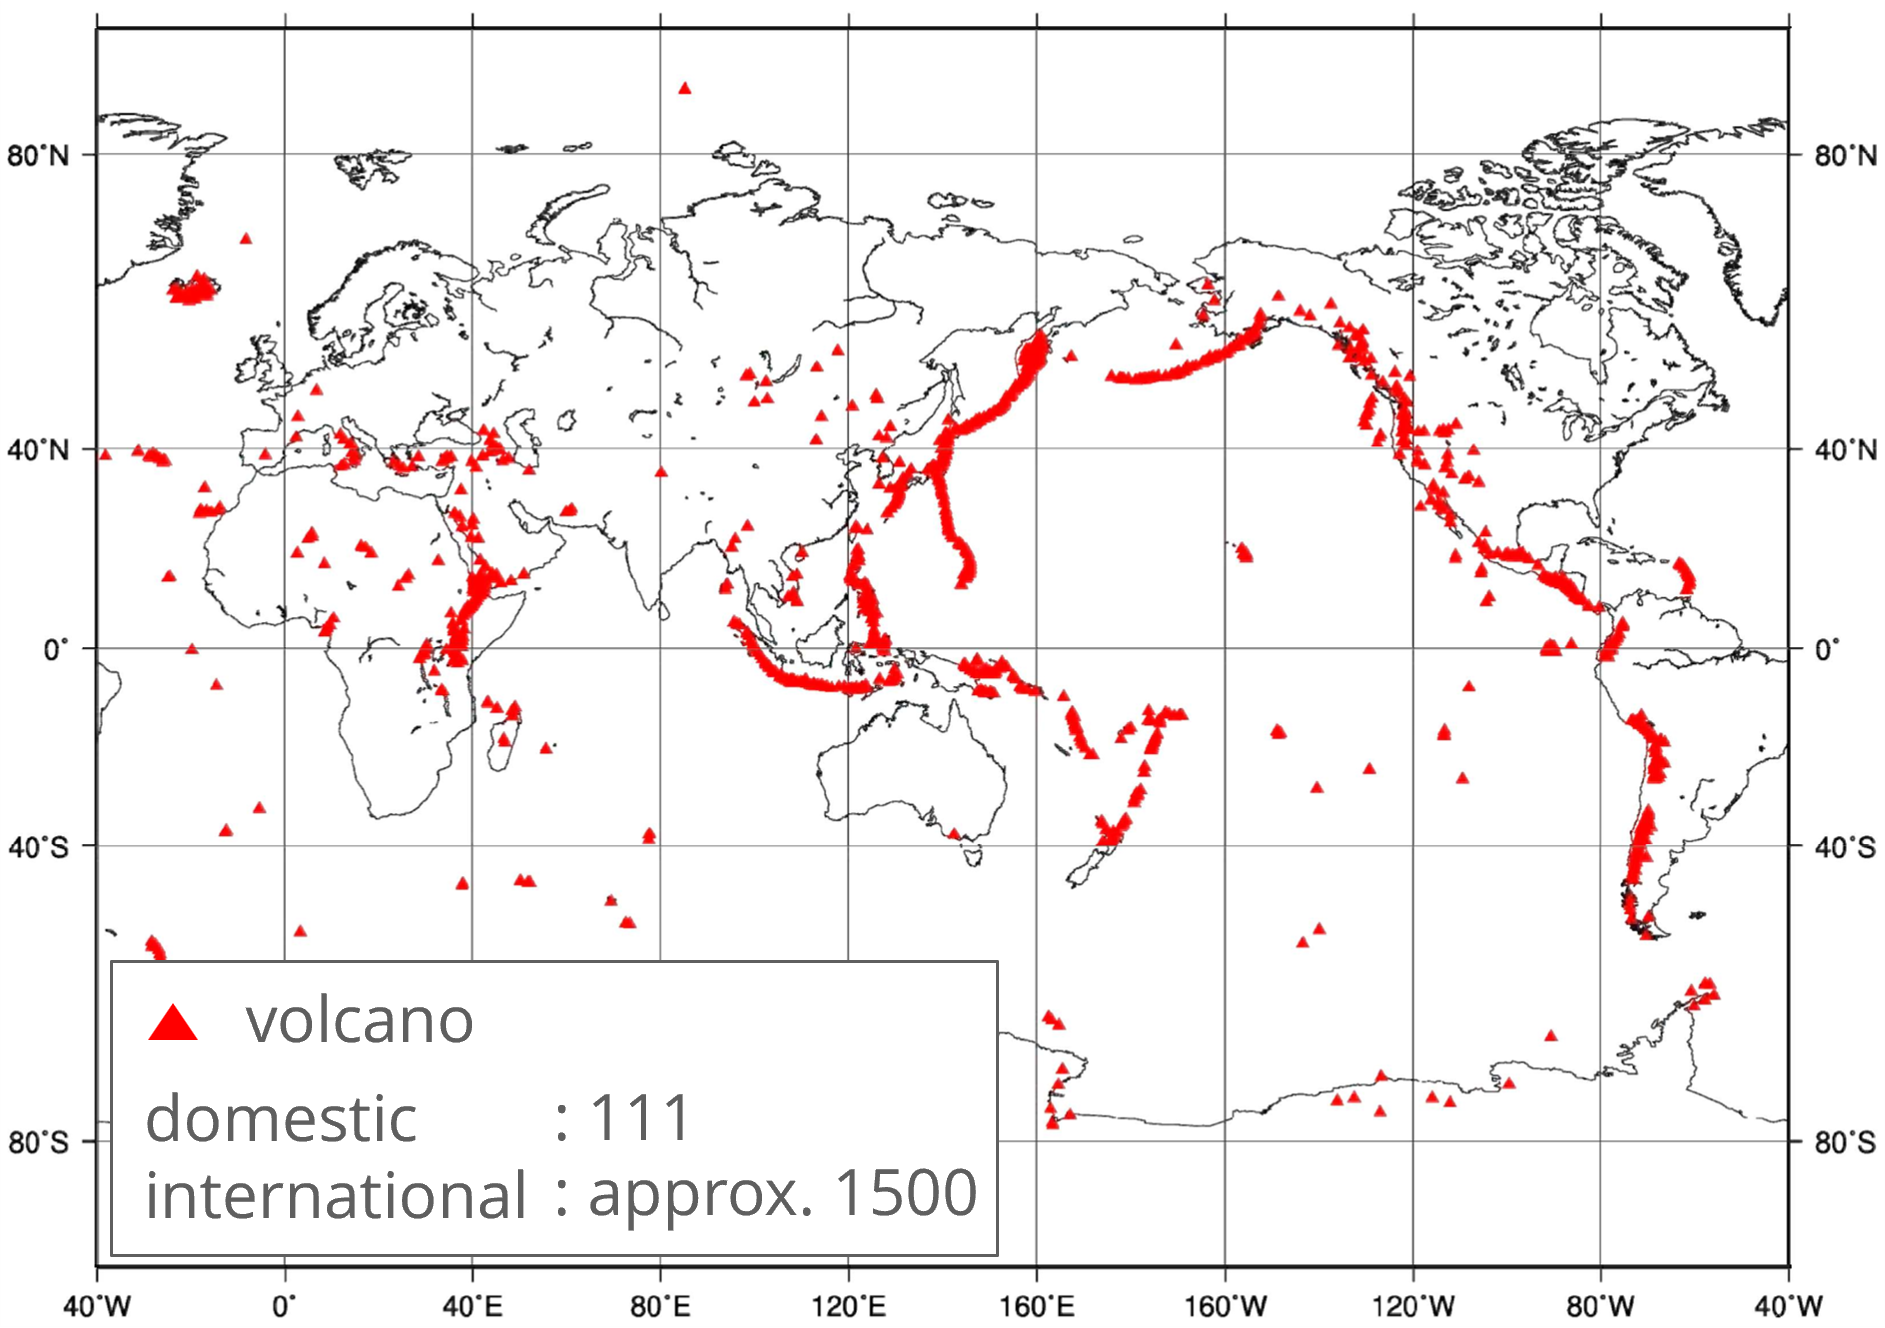
\includegraphics[width=0.6\linewidth]{fig/volcano_distribution.png}
    \caption{世界の活火山分布}
    \label{fig:volcano_dist}
\end{figure}

\newpage
火山災害には噴石や火砕流, 降灰など様々な形態が存在するが, 
火山ガスもまた重大な災害要因の一つである。過去100年間において,
火山ガスに起因する死亡者数は約1900人にのぼると報告されており,
火山ガスの危険性は決して小さくない\cite{Hirabayashi2003VolcanicGas}. 
火山ガスの中でも,二酸化硫黄（\ce{SO2}）は特に強い毒性を有する気体である. 
\cref{tab:SO2_toxicity}に\ce{SO2}の人体への影響を示す.
\begin{table}
    \centering
    \caption{二酸化硫黄の危険性}
    \label{tab:SO2_toxicity}
    \begin{tabular}{c|c}
        濃度[\unit{ppm}] & 人体への影響 \\
        \hline
        5 & 刺激症状（咳, 喉の痛み） \\
        30\sim40 & 呼吸困難 \\
        400\sim500 & 嗅覚が侵され, 臭気を知覚できない \\
        500 ppm\sim & 致死濃度\\
    \end{tabular}
\end{table}

\noindent
\ce{SO2}は,濃度が5 ppmを超えると呼吸器系への刺激が確認され,
30～40 ppmでは呼吸が困難となる. 
さらに,400 ppmを超える高濃度環境では生命に危険が及ぶことが知られている. 
その上, 強い毒性によって嗅覚が麻痺し, 特徴的な臭気を感知できなくなるため,
被害が拡大しやすいという性質も持ち合わせている.
実際, 環境基準としては, 環境基本法に基づき, 
% 「人の健康を保護し、生活環境を保全するうえで維持されることが望ましい基準」として
1時間値の1日平均値が\qty{0.04}{ppm}以下であり,
かつ, 1時間値が\qty{0.1}{ppm}以下であることと定められており, 
許容濃度としては, ACGIH\footnote{
    米国産業衛生専門家会議:American Conference of Governmental Industrial Hygienists
}が
通常の労働\footnote{
    1日8時間, 週40時間程度で肉体的に激しくない労働を指す. 
}
で, 平均暴露濃度が\qty{2}{ppm}以下であれば
ほとんどの労働者に健康上の悪い影響が見られないと判断している\cite{miyake}. 
平均暴露濃度は呼吸保護具を装着していない状態で
吸入するであろう濃度のことである. 
大気中の二酸化炭素濃度が約\qty{425}{ppm}前後であることを考えると,
\ce{SO2}が極めて低濃度で人体に深刻な影響を及ぼす強毒性ガスであることが分かる. 
加えて,\ce{SO2}は大気中で反応し,エアロゾルや硫酸ミストを形成する場合があり,
これらによる視程障害や呼吸器系への影響などの二次的被害も無視できない\cite{miyake}. 
そのため,三宅火山や霧島火山などでは,
火山性ガスの継続的な監視が実施されている。

\newpage
火山ガス観測には,電気化学式センサが広く用いられている. 
電気化学式センサは,測定対象ガスと触媒との電気化学反応量から気体濃度を推定する
微量気体濃度計であり,噴気が放出される地点に設置して測定が行われる. 
本手法は定点観測を前提としているため, 
気体濃度の空間分布を把握することができないという課題がある. 
また,反応が定常状態に達するまで濃度を評価できないことから,
時間的に連続した測定が困難であり,
人的被害を防ぐために継続して監視するにはこの課題も重要である.

\begin{figure}
    \centering
    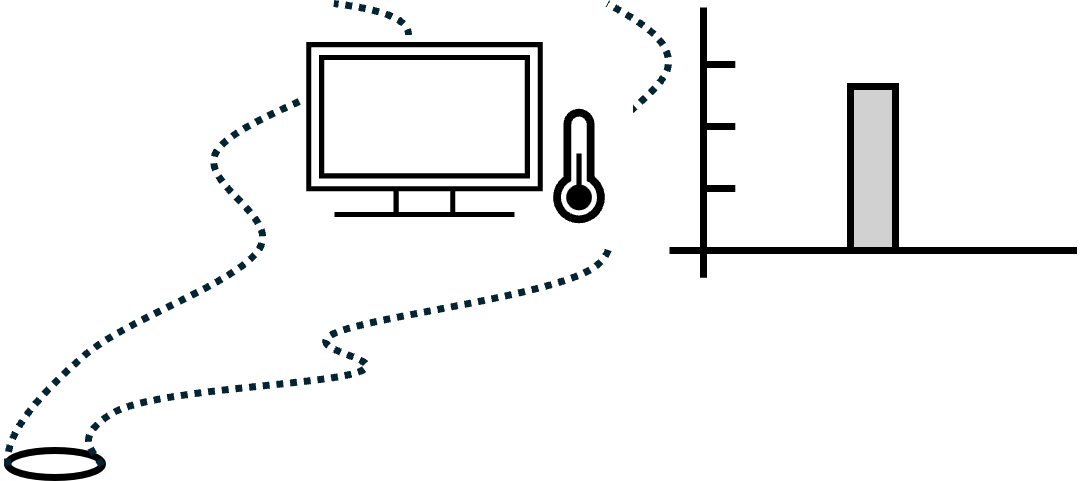
\includegraphics{fig/gassensor.png}
    \caption{電気化学式センサによる火山ガス観測イメージ}
    \label{fig:gassensor_image}
\end{figure}

これらの課題に対し, 微量気体を遠隔かつ空間分布, 
さらに時間連続的に観測する手法として, 
差分吸収ライダー（DIAL: Differential Absorption Lidar）
の利用が期待されている. 
DIALは, 測定対象気体に対して吸収特性の異なる2波長のレーザを照射し, 
その受信信号の差から濃度分布を推定する手法である. 
電気化学式センサと比較して, 
遠隔から周辺領域の濃度分布を時間的に連続して測定可能である点において優れている.

\begin{figure}
    \centering
    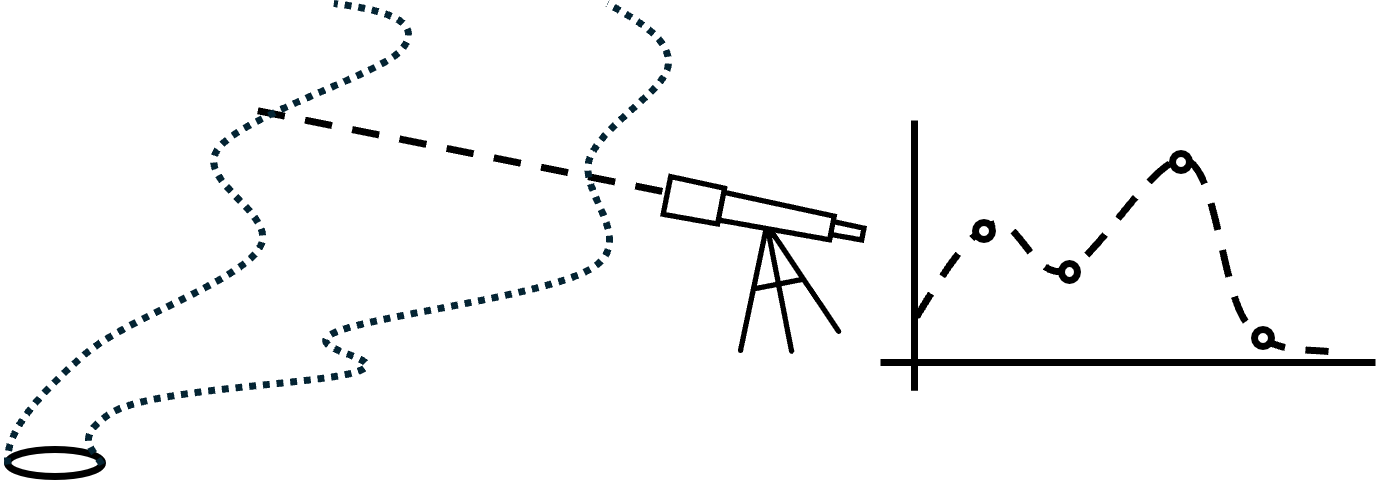
\includegraphics{fig/lidar.png}
    \caption{ライダーによる火山ガス観測イメージ}
    \label{fig:lidar_image}
\end{figure}

\newpage
\section{ラマンDIAL}
本研究で提案するラマンDIALは, 送信するレーザ波長によって生じる
ラマン散乱光をシステムに用いる受信波長として構成し, 
気体濃度の分布を測定する手法である. 
ラマン散乱とは, 
入射したレーザ光が分子の振動エネルギー準位と相互作用することで, 
入射光とは異なる波長成分を持つ散乱光が生成される現象である.
また, ラマン散乱には長波長側にシフトするストークス散乱と, 
短波長側にシフトするアンチストークス散乱が存在し, 
一般的にアンチストークス散乱の強度はストークス散乱と比較して 
1/10 以下と非常に微弱である. 
\cref{fig:ramanDIAL}にラマンDIALの基本的な構成を示す. 
\begin{figure}
    \centering
    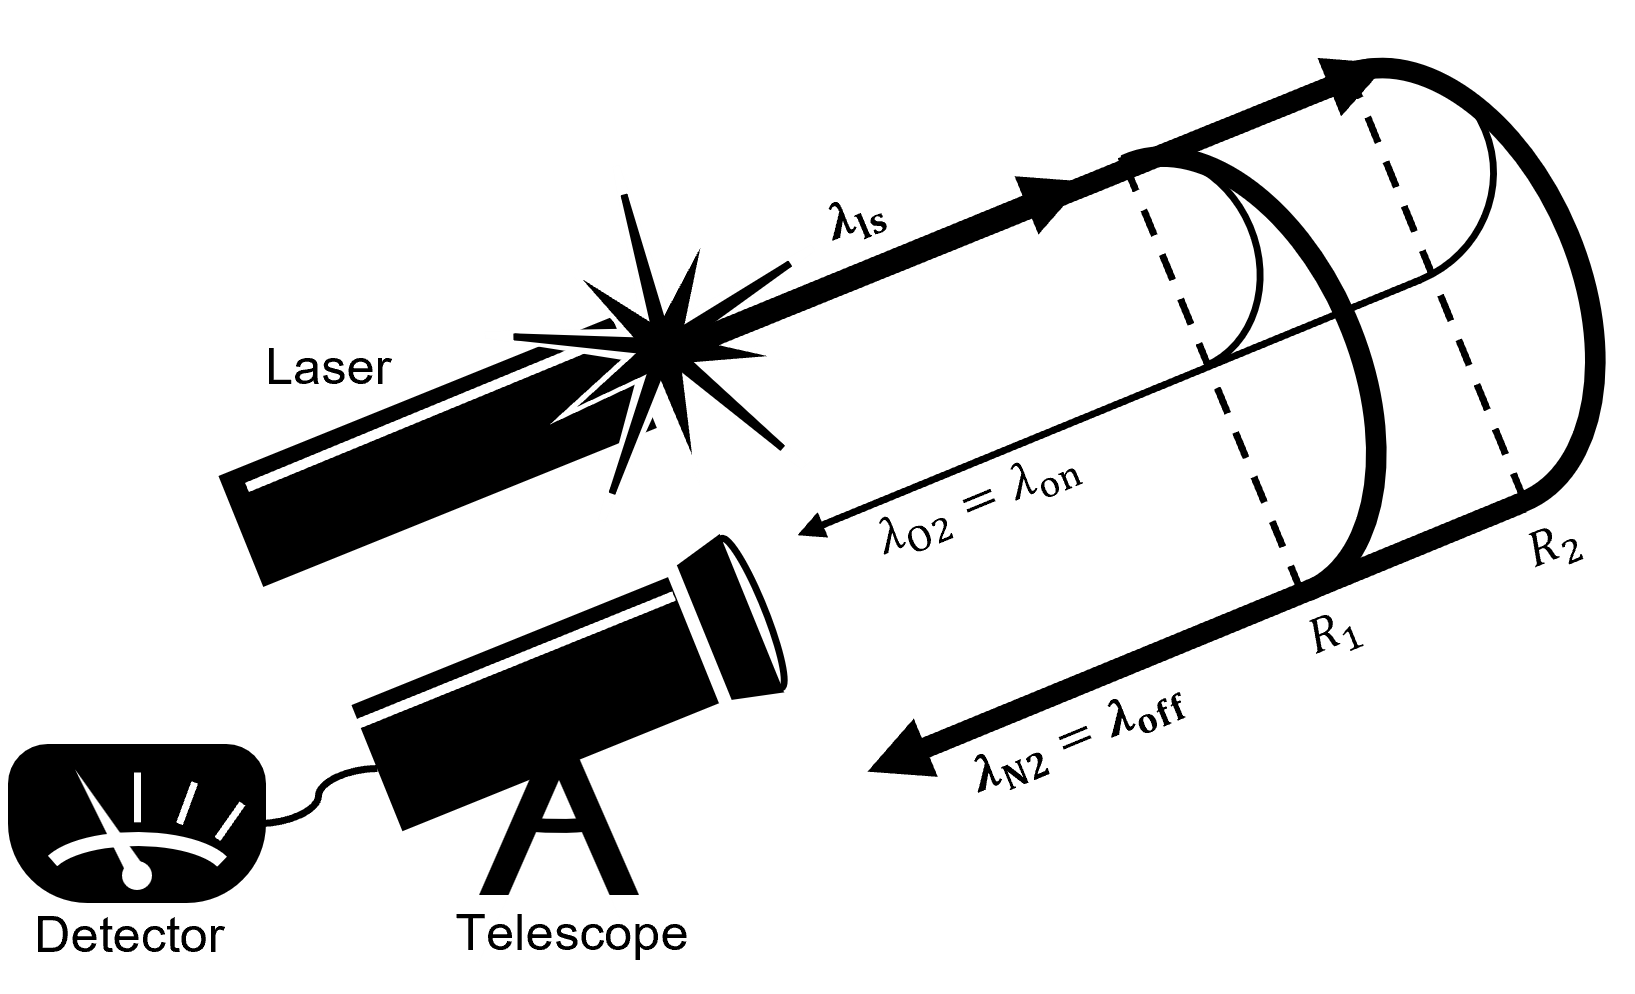
\includegraphics[width=0.8\linewidth]{fig/ramanDIAL.png}
    \caption{ラマンDIAL構成図}
    \label{fig:ramanDIAL}
\end{figure}

\noindent
今回提案するラマンDIALは大気中の酸素分子（\ce{O2}）及び窒素分子(\ce{N2})のラマン散乱を利用する. 
\ce{O2}のラマンシフトは\qty{1556}{cm^{-1}}, 
\ce{N2}のラマンシフトは\qty{2331}{cm^{-1}}であり, 
それぞれのラマン散乱波長はレーザ波長に対して, 
このラマンシフト分だけ波長変化することになる. 
ここで, 対象気体の吸収が強い波長をオン波長\subrm{\lambda}{on}, 
吸収が弱い波長をオフ波長\subrm{\lambda}{off}と呼ぶ. 
この手法の特徴は, 通常のDIALに対して, 送信レーザの波長数を削減し, 
受信側で2波長を構成できることであり, 
これによりシステムの小型化が期待される.

\newpage
ライダー視線上の距離$R$におけるライダーの受信光子数\subrm{P}{phot}は
\cref{equ:power,equ:alpha}で求められる\cite{PowerEqu}. 
\begin{align}
    P(R)
    &=\frac{E_0}{h\subrm{\lambda}{ls}}
    M \eta q \Delta R \frac{A}{R^2}O(R) \subrm{\beta}{ram}
    \exp\ab[
        \int^{R}_{0}
            \ab(
                \alpha(r, \subrm{\lambda}{ls})
                +\alpha(r, \subrm{\lambda}{ram})
            )\dd r 
    ]\label{equ:power}\\
    \alpha(\lambda, r) 
    &= \subrm{\alpha}{air}(\lambda)
    +\sum^{N}_{\mathrm{gas}=1}
        \subrm{n}{gas}(r)\subrm{\sigma}{gas}(\lambda)\label{equ:alpha}
\end{align}

\noindent
式中の$E_0$はパルスエネルギー, 
$h$はプランク定数, 
$M$は積算回数, 
$q$は光学系の全効率, 
$\eta$はディテクターの量子効率, 
$\Delta R$は距離分解能, 
$A$は受信鏡直径
$O(R)$は重なり関数を表す. 
後方ラマン散乱断面積\subrm{\beta}{ram}について,
清水らが報告した結果から, 
窒素の\subrm{\beta}{ram}は\qty{2.8e-34}{m^2}, 
酸素の\subrm{\beta}{ram}は\qty{3.9e-34}{m^2}とした\cite{ramanXS}. 
そして, これを0.1した値をアンチストークス散乱の後方散乱断面積とした. 
% 式中の$C$はライダーのシステムパラメータ, 
% $\beta_{ram}$は後方ラマン散乱断面積,  
% $\lambda_{\mathrm{ls}}$はレーザ波長, 
% $\lambda_{\mathrm{ram}}$はラマン散乱波長である.  
\cref{equ:alpha}に示す消散係数$\alpha$は, 大気及び各種気体による吸収の総和であり, 
ここでgas=1,2,…,Nはガス成分の種類を表す. 

距離$R_1, R_2(R_1<R_2)$における2波長\subrm{\lambda}{on}, 
\subrm{\lambda}{off}のライダーの受信光子数から\ce{SO2}の濃度分布は
\cref{equ:n_SO2}で求められる\cite{DIALEqu}.
\Delta\sigma はon波長とoff波長における
\ce{SO2}吸収断面積の差分である. 
\begin{equation}
    \subrm{n}{SO2}
    =\frac{1}{\Delta\subrm{\sigma}{SO2}\Delta R}\ln\ab(
        \frac
        {P(\subrm{\lambda}{on}, R_1)P(\subrm{\lambda}{off}, R_2)}
        {P(\subrm{\lambda}{on}, R_2)P(\subrm{\lambda}{off}, R_1)}
    )\label{equ:n_SO2}
    % \Delta\sigma_{\mathrm{SO2}} &= 
    % \sigma_{\mathrm{SO2}}(\lambda_{\mathrm{on}})-
    % \sigma_{\mathrm{SO2}}(\lambda_{\mathrm{off}})
\end{equation}

% \begin{table}[t]
%   \centering
%   \caption{System parameters for Raman DIAL.}
%   \label{tab:system_parameters}
%   \begin{tabular}{c p{60mm} p{20mm}}
%     \hline
%     $E_0$ [mJ] & Pulse energy & 30 \\
%     $A$ [m] & Diameter of the telescope & 0.6 \\
%     $M$ & Number of integration times & $100 \si{Hz}\times$30 \si{min} \\
%     $\eta$ & Quantum efficiency of the detector & 0.3 \\
%     $q$ & Total efficiency of optics & 0.3 \\
%     $\Delta R$ [m] & Spatial resolution & 30 \\

%     % $\sigma_{\mathrm{RamanN2}}$ [m$^2$] &
%     % Stokes Raman scattering cross section of N$_2$ &
%     % $2.8 \times 10^{-34}$ \\

%     % $\sigma_{\mathrm{RamanO2}}$ [m$^2$] &
%     % Stokes Raman scattering cross section of O$_2$ &
%     % $3.9 \times 10^{-34}$ \\

%     % $\sigma'_{\mathrm{ramN2}}$ [m$^2$] &
%     % anti-Stokes Raman scattering cross section of N$_2$ &
%     % $2.8 \times 10^{-35}$ \\

%     % $\sigma'_{\mathrm{ramO2}}$ [m$^2$] &
%     % anti-Stokes Raman scattering cross section of O$_2$ &
%     % $3.9 \times 10^{-35}$ \\
%     \hline
%   \end{tabular}
% \end{table}

\section{本研究の目的}
本研究は, ラマンDIALの遠隔・分布・時間的連続観測に着目し, 
火山ガス中の\ce{SO2}の測定への適応可能性を数値シミュレーションにより
検証することを目的とする.
目安として, \ce{SO2}濃度に対する±\qty{10}{\%}の測定誤差を基準に設定した. 

本研究の新規性として, 
信号強度の課題からこれまで十分検討されてこなかった
アンチストークス散乱信号に注目し, 
アンチストークス散乱波長を含む受信波長構成と
従来構成を定量的に比較した点が挙げられる. 
